% !TEX root = main.tex
\chapter{実験結果}
本章では3.1節ではブロードコンタクトレーザー、3.2節ではリッジ導波路型レーザーへの電流注入実験についての結果を報告する。
\section{ブロードコンタクトレーザー試料に関する測定結果}%=====================================
ブロードコンタクトレーザーへ定常電流を流してILカーブを得る実験を行った。様々な共振器長L、電極パッド幅wの試料に対して実験を行うことでウエハの基本的な物性パラメータを見積もることが目的である。

具体的には発振閾値電流$I_{\rm{th}}$を測定することに加えて、発振時の印可電流の増分に対する光出力の増大から発光量子効率(微分外部量子効率)を見積もることが目的である。
また発振閾値電流密度を算出するためにデバイス内の電流の広がりを見積もった。
3周期ウエハと10周期ウエハごとに節を分けている。
\subsection{3周期歪量子井戸ブロードコンタクトレーザー}%===============================
3周期量子井戸ブロードコンタクトレーザーの結果を示す。図\ref{fig:fig_3_1_3QW_broacdcontact_IL}(a)縦軸に発光強度(片方の端面)、横軸に電流をとったILカーブの結果を示す。また\ref{fig:fig_3_1_3QW_broacdcontact_IL}(b)は縦軸に試料にかかっている電圧、横軸に電流をとったIVカーブの結果である。共振器長LがL=500,1000,2000umの結果をプロットした。代表としてパッド幅w=50umの結果をプロットした。印可電流は1usパルスを2ms繰り返し周期で流しており、デューティー比は1:2000である。

\begin{figure}[h]
	\centering
	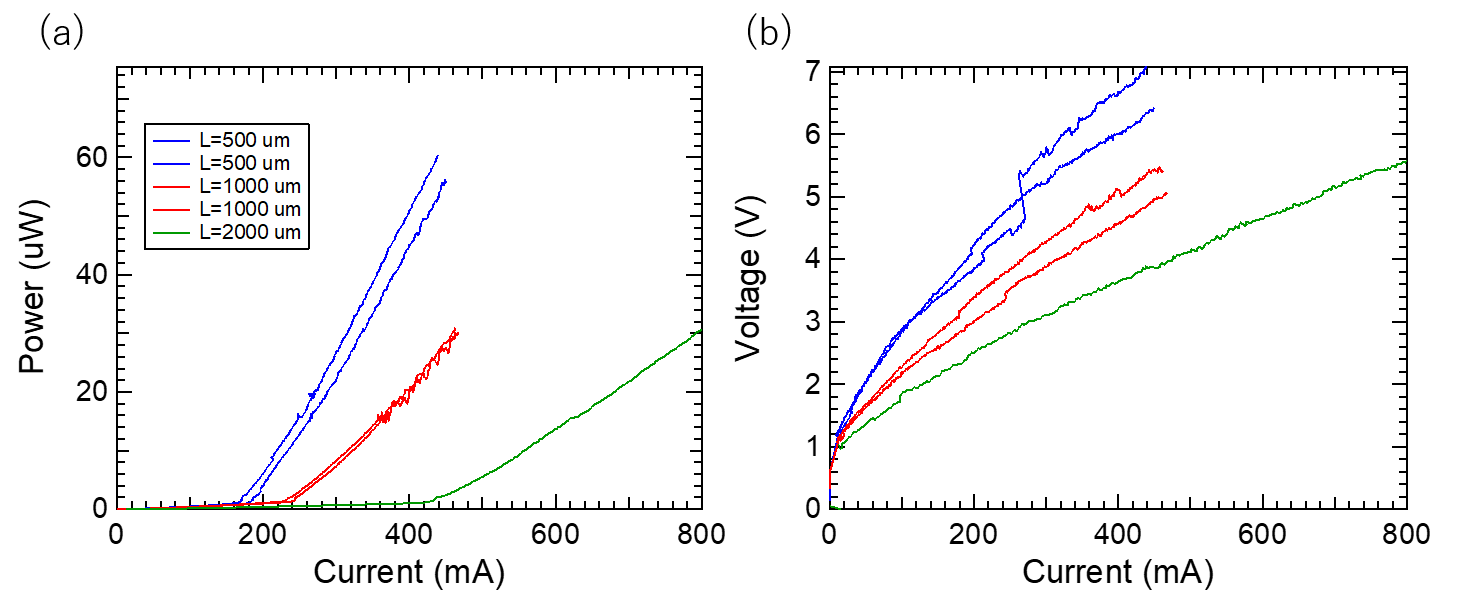
\includegraphics[width=15cm]{figure/fig_3_1_3QW_broadcontact_IL.png}
		\caption{3周期歪量子井戸ブロードコンタクトレーザーのILカーブとIVカーブ}
		\label{fig:fig_3_1_3QW_broacdcontact_IL}
\end{figure}

(a)を見ると各デバイスにおいて光出力強度が電流値を上げてくと増加していき、ある電流値を超えると発振が始まり発光強度が急激に増加することがわかる。その電流値を発振しているときのILカーブを直線フィッティングすることで求めた。フィッティング直線のx切片を発振閾値電流$I_{\rm{th}}$とした。またフィッティング直線の傾きを発振時のスロープ効率$\Delta P/\Delta I$とした。スロープ効率はフィッティングの傾きにデューティー比をかけ、共振器の両端面からの放出を考慮して2倍にして算出した。
典型的な値として、図\ref{fig:fig_3_1_3QW_broacdcontact_IL}(a)のILカーブの値を表\ref{table:table_3_1_3QW_broadcontact}に示す。表では
\begin{table}[h]
  \caption{3周期ブロードコンタクトレーザーの閾値電流}
  \label{table:table_3_1_3QW_broadcontact}
  \centering
  \begin{tabular}{ccc}
    \hline
    共振器長L(um)  & 閾値電流$I_{th}$ (mA)  & Slope 2$\Delta P/\Delta I$ (W/A) \\
    \hline \hline
     500& 187&  0.83  \\
    1000& 234& 0.51\\
    2000& 450&0.37\\
       \hline
  \end{tabular}
\end{table}



\ref{fig:fig_3_1_3QW_broacdcontact_IL}(b)を見ると各デバイスにおいて電流が流れ始めるのが1V付近からでありダイオード特性が見られる。また共振器長Lが長いほど同じ電流に対する電圧が低い。これは共振器長Lに比例して電流が流れる面積が大きくなるためデバイスの抵抗値が小さくなっているためである。


次に様々なパッド幅に対して見積もった発振閾値電流$I_{\rm{th}}$の結果を図\ref{fig:fig_3_1_3QW_broadcontact_Ith}(a)に示す。発振閾値電流$I_{\rm{th}}$、横軸が電極パッド幅wである。\ref{fig:fig_3_1_3QW_broadcontact_Ith}(b)は発振時の発光効率$2 \Delta P/\Delta I$である。

図\ref{fig:fig_3_1_3QW_broadcontact_Ith}(a)を見ると、パッド幅wが50umより大きい領域では閾値電流$I_{\rm{th}}$はパッド幅wに対して線形に増加していることがわかる。一方パッド幅wが小さい領域では線形に変化していない。

この原因は電流がパッド幅wに対して無視できないほど広がってしまっているためだと考えられる。電流広がりについてはフィッティングから見積もった。詳しくは3.1.3節で述べる。

図\ref{fig:fig_3_1_3QW_broadcontact_Ith}(b)を見るとそれぞれの共振器長で概ね横ばいの値を持っている。$\Delta P/\Delta I$はパッド幅wに依存しないことがわかる。幅wは光の増幅を受ける方向とは関係がなく、直感と一致する。

\begin{figure}[h]
	\centering
	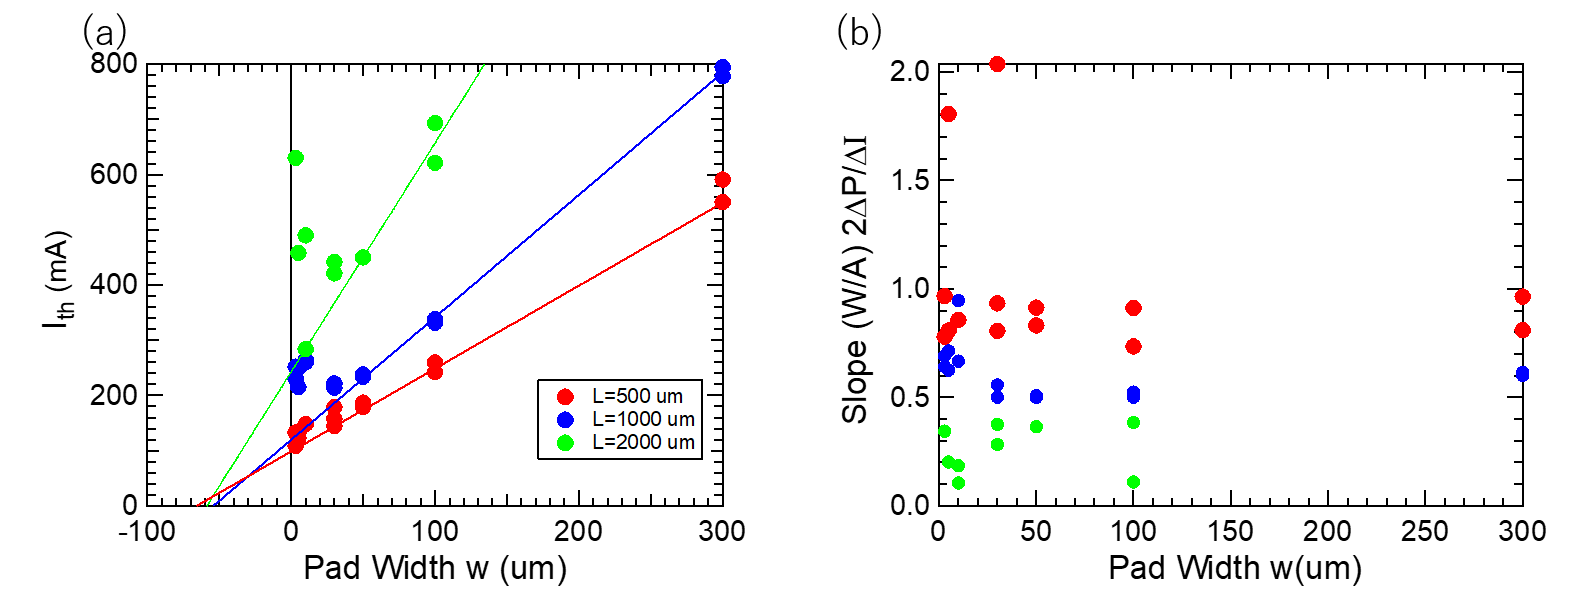
\includegraphics[width=15cm]{figure/fig_3_1_3QW_broadcontact_Ith.png}
		\caption{3周期歪量子井戸ブロードコンタクトレーザーの閾値電流と発光効率}
		\label{fig:fig_3_1_3QW_broadcontact_Ith}
\end{figure}
\clearpage
\subsection{10周期歪補償量子井戸ブロードコンタクトレーザー}%===============================
次に10周期歪補償量子井戸ブロードコンタクトレーザーについての結果を示す。図\ref{fig:fig_3_1_10QW_broadcontact_IL}(a)にILカーブ、(b)にIVカーブを示す。w=50umを代表としてプロットした。色分けは共振器長の違いを表す。電流は2usパルスを2ms繰り返し周期で印可した。デューティー比は1:1000である。
\begin{figure}[h]
	\centering
	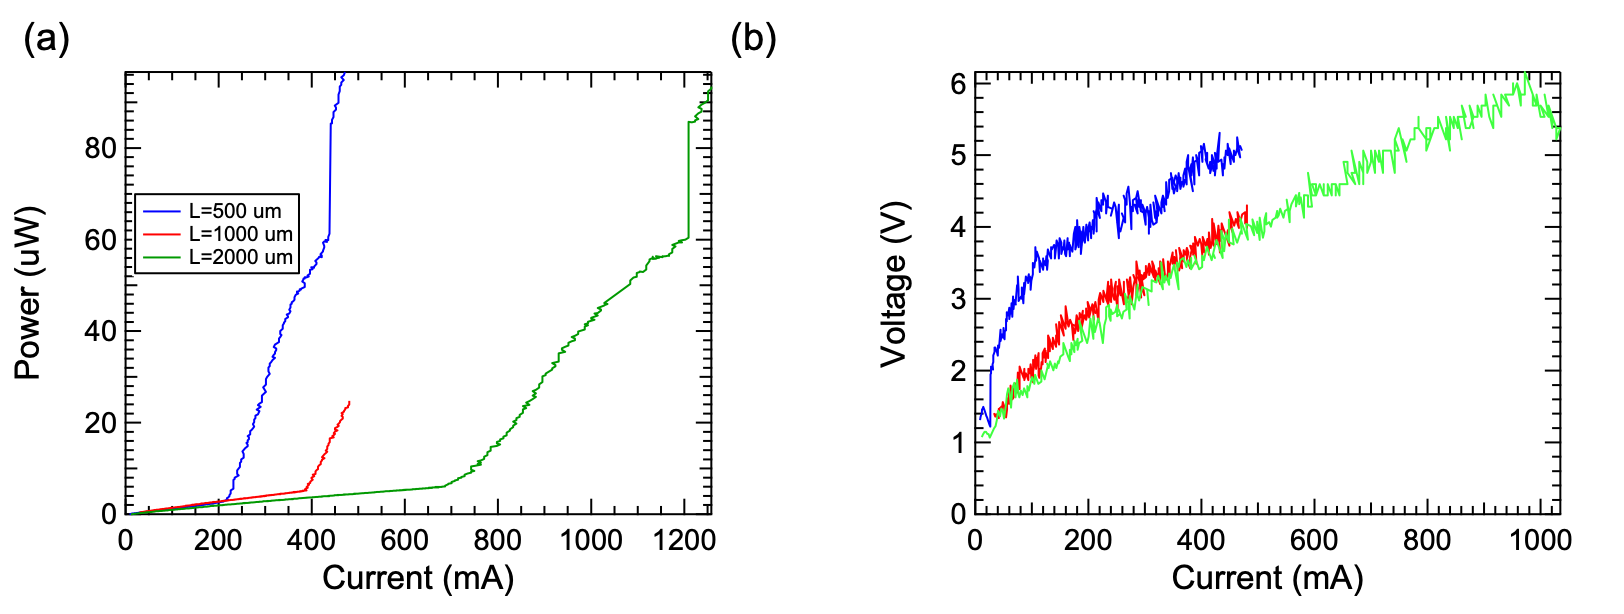
\includegraphics[width=15cm]{figure/fig_3_1_10QW_broadcontact_IL.png}
		\caption{10周期歪補償ブロードコンタクトレーザーのILカーブとIVカーブ}
		\label{fig:fig_3_1_10QW_broadcontact_IL}
\end{figure}

典型的な値として図
\ref{fig:fig_3_1_10QW_broadcontact_IL}(a)のILカーブフィッティング結果の値を表\ref{table:table_3_1_10QW_broadcontact}に示す。傾きはデューティー比1:1000と両端面からの発光を換算していることに注意されたい。
\begin{table}[h]
  \caption{10周期歪補償ブロードコンタクトレーザーの閾値電流}
  \label{table:table_3_1_10QW_broadcontact}
  \centering
  \begin{tabular}{ccc}
    \hline
    共振器長L(um)  & 閾値電流$I_{th}$ (mA)  & Slope 2$\Delta P/\Delta I$ (W/A) \\
    \hline \hline
     500& 212&  0.64  \\
    1000& 363& 0.42\\
    2000& 501&0.27\\
       \hline
  \end{tabular}
\end{table}

次に\ref{fig:fig_3_1_3QW_broadcontact_Ith} (a)に\ref{fig:fig_3_1_10QW_broadcontact_IL} (a)のILカーブの発振時の直線フィッティング結果から求めた閾値電流$I_{\rm{th}}$および(b)スロープ効率2 $\Delta P/\Delta I$をパッド幅wに対してプロットした。
\begin{figure}[h]
	\centering
	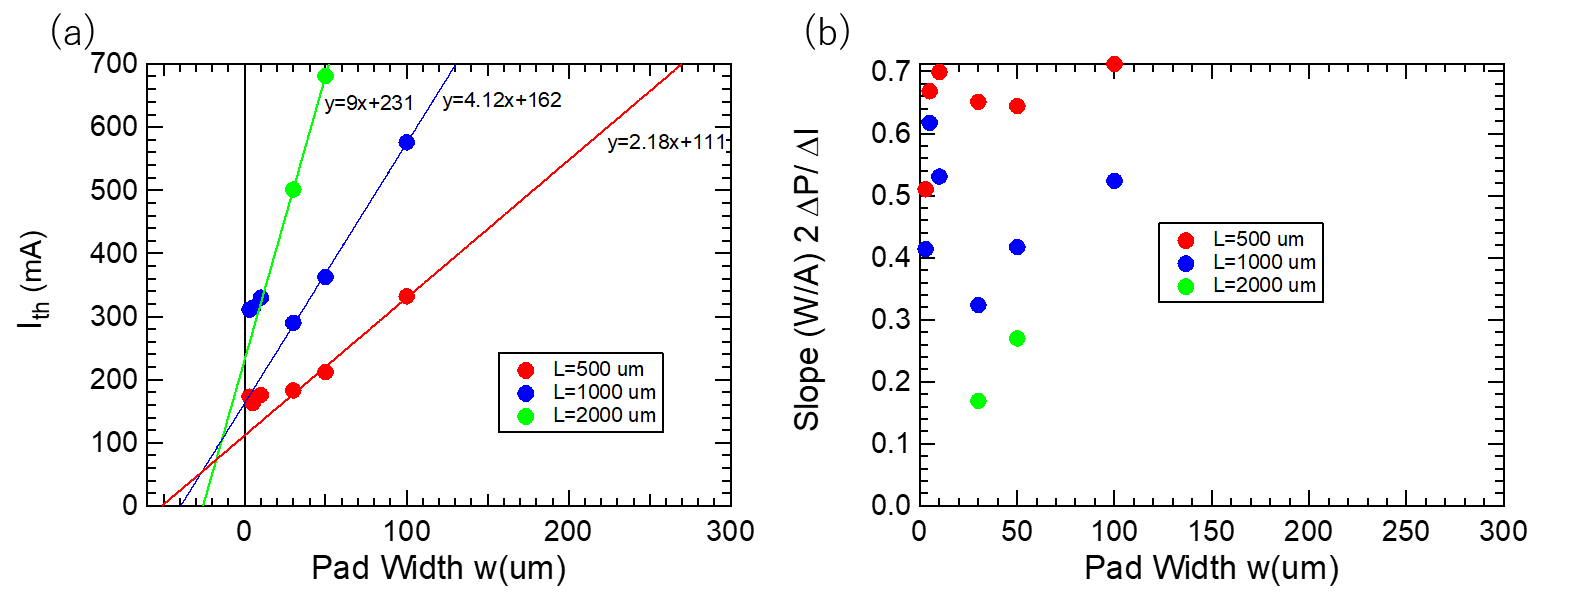
\includegraphics[width=15cm]{figure/fig_3_1_10QW_broadcontact_Ith.png}
		\caption{10MQWのIL結果}
		\label{fig:fig_3_1_10QW_broadcontact_Ith}
\end{figure}

\subsection{電流広がりに関する考察}%==================
3.1.1節と3.1.2節でILカーブから3周期歪量子井戸ブロードコンタクトレーザーと10周期歪補償ブロードコンタクトレーザーについて閾値電流$I_{\rm{th}}$を見積もった。この値から閾値電流密度$J_{\rm{th}}$を求めることが大切である。
レーザーの基本的な特性を知る上で閾値電流密度が大切なパラメータであるからである。発振閾値電流$I_{\rm{th}}$を電流が流れた面積で割ることで閾値電流密度$J_{\rm{th}}$が求まる。

通常閾値電流$I_{\rm{th}}$は電流を流す面積に比例して大きくなる。面積とは電極パッド幅wと共振器長Lの積で表される。つまり$I_{\rm{th}}$はwに対して線形に増加するはずである。しかし図\ref{fig:fig_3_1_3QW_broacdcontact_IL} (a)や\ref{fig:fig_3_1_10QW_broadcontact_IL}(a) を見るとそうなっていない。そこで発振閾値電流$I_{\rm{th}}$が線形に増加する領域を直線フィッティングし、その直線のx切片を含めたパッド幅を有効的なパッド幅と考えて閾値電流密度を算出した。まずは有効パッド幅を見積もった。フィッティング関数のx切片の絶対値が実質的なパッド幅の増分w'である。その値を表\ref{table:table_3QW_broadcontact_w_eff}と表\ref{table:table_10QW_broadcontact_w_eff}に示した。
\begin{table}[h]
  \caption{3周期歪量子井戸ブロードコンタクトレーザーの電流広がり}
  \label{table:table_3QW_broadcontact_w_eff}
  \centering
  \begin{tabular}{cc}
    \hline
    共振器長L (um)  & パッド幅の増分(電流の広がり) w' (um)   \\
    \hline \hline
     500 & 65.8  \\
    1000  & 54.1 \\
    2000  & 58.7 \\ 
    \hline
  \end{tabular}
\end{table}

\begin{table}[h]
  \caption{10周期歪補償ブロードコンタクトレーザーの電流広がり}
  \label{table:table_10QW_broadcontact_w_eff}
  \centering
  \begin{tabular}{cc}
    \hline
    共振器長L (um)  & パッド幅の増分(電流の広がり) w' (um)   \\
    \hline \hline
     500 & 51.1  \\
    1000  & 39.5 \\
    2000  & 25.7 \\ 
    \hline
  \end{tabular}
\end{table}

3QWでは58umから65um程度の広がりであることが見積もられた。10QWでは値のばらつきが大きくL=500のw'とL=2000umのw'を比較すると2倍程度異なってしまっている。これは共振器の長い試料について、wが大きい試料に対しての実験結果がないため、w'の見積もりが小さくなってしまったためであると考えられる。
この表の値w'と閾値電流$I_{\rm{th}}$(mA)から式(\ref{eq:Jth})の関係を用いて閾値電流密度$J_{\rm{th}} \rm{(kA/cm^2)}$を算出した。
\begin{eqnarray}
J_{\rm{th}}=\dfrac{I_{\rm{th}}}{(w+w')L}
\label{eq:Jth}
\end{eqnarray}

その結果を示す。図\ref{fig:fig_3_1_3QW_broadcontact_Ith}に3周期歪量子井戸ブロードコンタクトレーザーの結果、\ref{fig:fig_3_1_10QW_broadcontact_Ith}に10周期歪補償量子井戸ブロードコンタクトレーザーの結果をプロットした。

\begin{figure}[h]
	\centering
	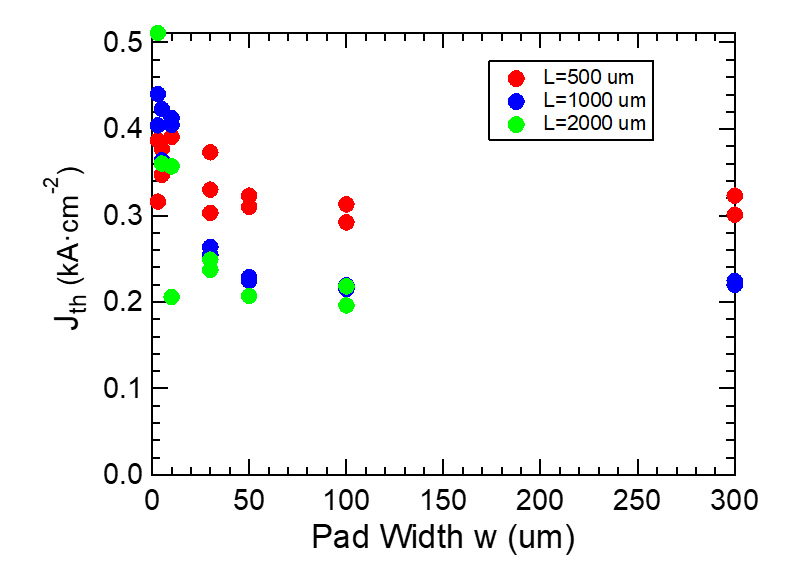
\includegraphics[width=10cm]{figure/fig_3_1_3QW_broadcontact_Jth.png}
		\caption{3周期歪量子井戸ブロードコンタクトレーザーの閾値電流密度}
		\label{fig:fig_3_1_3QW_broadcontact_Jth}
\end{figure}

\begin{figure}[h]
	\centering
	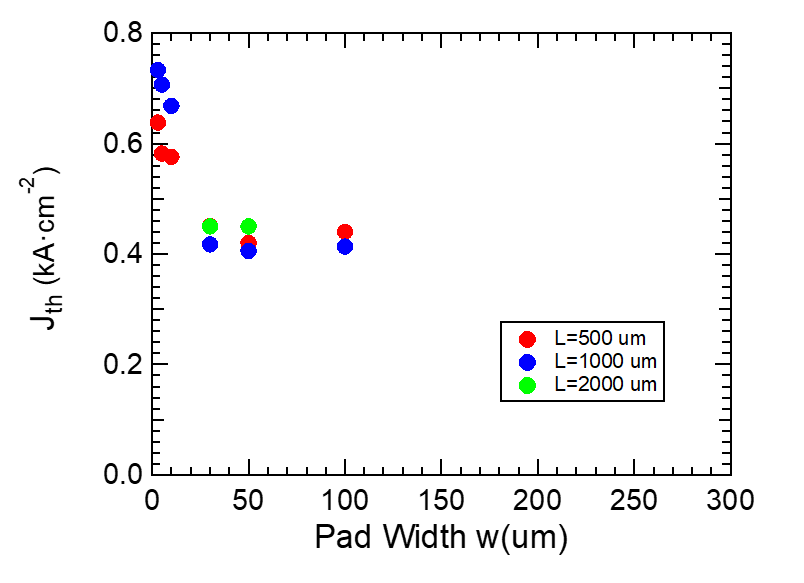
\includegraphics[width=10cm]{figure/fig_3_1_10QW_broadcontact_Jth.png}
		\caption{10周期歪補償量子井戸ブロードコンタクトレーザの閾値電流密度}
		\label{fig:fig_3_1_10QW_broadcontact_Jth}
\end{figure}
3周期歪量子井戸ブロードコンタクトレーザーでは$0.20\sim 0.35 \rm{(kA/cm^{2})}$、10周期歪補償ブロードコンタクトレーザーでは$0.40 \rm{(kA/cm^{2})}$程度と見積もられた。

3QWでは wが50より大きい領域で、共振器長が長くなるほどJthが小さくなることがわかる。これは共振器長が長くなるほどミラーロスに対する内部ロスが大きくなっていき、発振が起こりにくくなっているためである。

一方10QWではL=2000umの値が他の2つに比べて大きくなってしまっている。これはw'が小さく見積もられており、Jthが大きく見積もられたためだと考えられる。w'の解析に用いたプロット点数が少ないことが原因である。
\clearpage
\subsection{外部量子効率、内部量子効率と吸収係数の計算}%=============
次にILカーブの発振時の傾きに相当するスロープ効率$\Delta P/\Delta I$から試料の内部微分量子効率$\eta_{i}$および吸収係数$\alpha$を算出した。まずはスロープ効率$2 \Delta P/\Delta I \rm{(W/A)}$から外部微分量子効率$\eta_{\rm{d}}$を算出した。式({\ref{eq:eta_d})の関係を用いた。
\begin{eqnarray}
\eta_{\rm{d}}=\dfrac{e}{h\nu}2\dfrac{\Delta P}{\Delta I} 
\label{eq:eta_d}
\end{eqnarray}
eは電気素量、hはプランク定数、$\nu$は発振周波数であり、1050nmとした。$\eta_{\rm{d}}$はキャリアの注入数に対する取り出せる光子の数の割合である。結果を図\ref{fig:fig_3_1_3QW_broadcontact_id}に示す。縦軸を$\eta_{\rm{d}}$横軸をパッド幅wとしてプロットした。色分けが共振器長の違いを表している。L=500umでは0.7程度、L=1000umでは0.4程度、L=400umでは0.3程度の値を持っている。
\begin{figure}[h]
	\centering
	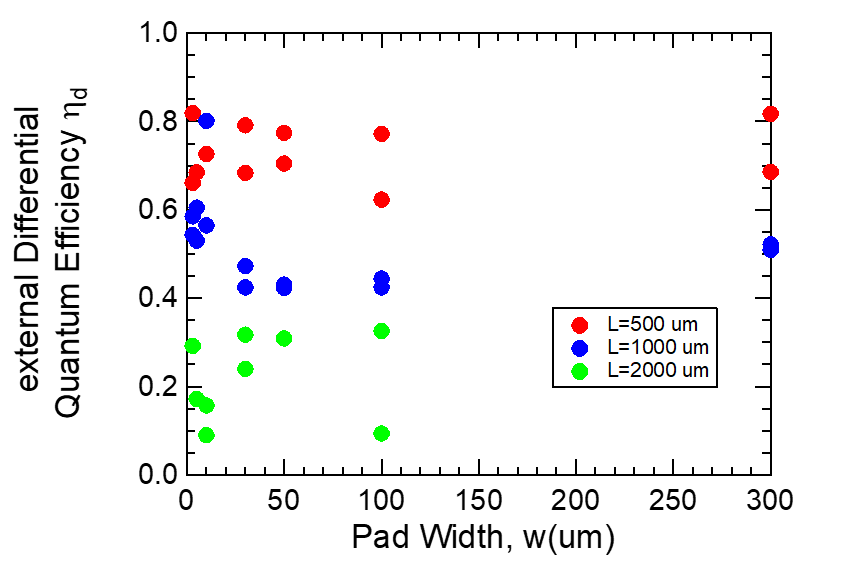
\includegraphics[width=10cm]{figure/fig_3_1_3QW_broadcontact_id.png}
	\caption{3周期歪量子井戸ブロードコンタクトレーザーの外部量子効率}
	\label{fig:fig_3_1_3QW_broadcontact_id}
\end{figure}


$\eta_{\rm{d}}$は共振器長Lを用いて式(\ref{eq:eta_inverse})と書き表される。
\begin{eqnarray}
\dfrac{1}{\eta_{\rm{d}}}=\dfrac{\alpha_{\rm{int}}}{\rm{ln}(1/R)\eta_{int}}L+\dfrac{1}{\eta_{\rm{int}}}
\label{eq:eta_inverse}
\end{eqnarray}
$\alpha_{int}$は共振器内の平均の内部損失、Rは共振器の端面での反射率、$\eta_{\rm{int}}$は内部微分量子効率である。Rは半導体デバイスの屈折率と空気の屈折率の差から0.32と仮定した。見積もった$\eta_{\rm{d}}$の逆数を共振器長に対してプロットし直線フィッティングを行なった。これを図\ref{fig:fig_3_1_3QW_broadcontact_id_inverse}に示す。横軸は共振器長L、縦軸に外部微分量子効率の逆数$1/\eta_{\rm{d}}$である。例としてパッド幅w=100umの結果を示す。式(\ref{eq:eta_inverse})よりこのフィッティング直線のy切片から内部量子効率$\eta_{\rm{int}}$を見積もると$\eta_{\rm{int}}$=0.96と計算できる。また、直線の傾きから内部損失$\alpha_{\rm{int}}$を見積もると$\alpha_{\rm{int}}$=11.8 (/cm)と計算できた。
\begin{figure}[h]
	\centering
	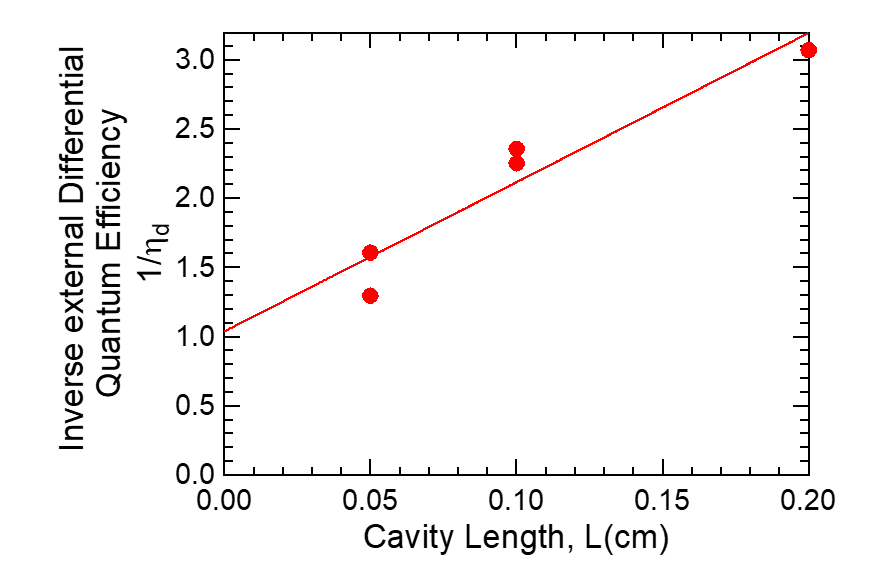
\includegraphics[width=10cm]{figure/fig_3_1_3QW_broadcontact_id_inverse.png}
	\caption{3周期歪量子井戸レーザーの外部量子効率の逆数}
	\label{fig:fig_3_1_3QW_broadcontact_id_inverse}
\end{figure}



\newpage

同様の解析を10周期歪補償量子井戸ブロードコンタクトレーザーの結果についても行った。図\ref{fig:fig_3_1_10QW_broadcontact_id}に外部微分量子効率、図\ref{fig:fig_3_1_10QW_broadcontact_id_inverse}こちらはw=50um の結果を示している。10周期に関しては$\eta_{\rm{int}}$=0.94、$\alpha_{\rm{int}}$=18.0 (/cm)となった。
\begin{figure}[h]
	\centering
	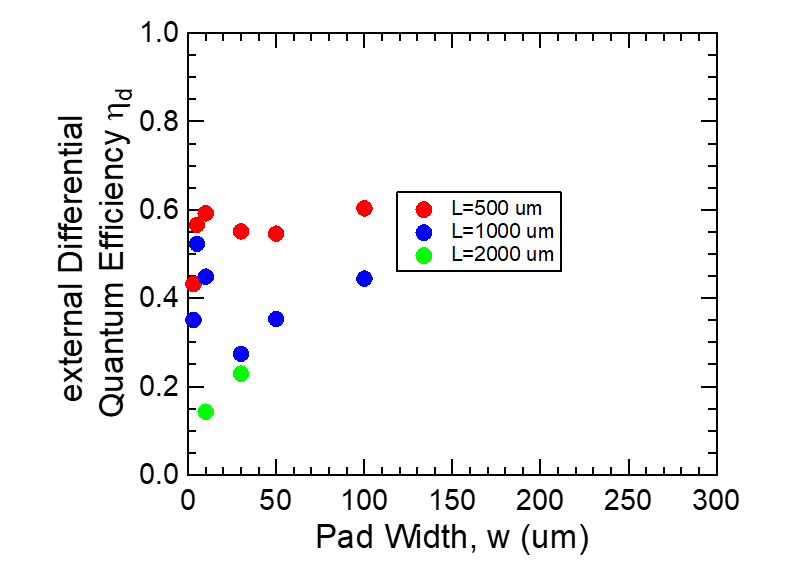
\includegraphics[width=10cm]{figure/fig_3_1_10QW_broadcontact_id.png}
	\caption{10QW外部量子効率}
	\label{fig:fig_3_1_10QW_broadcontact_id}
\end{figure}

\begin{figure}[h]
	\centering
	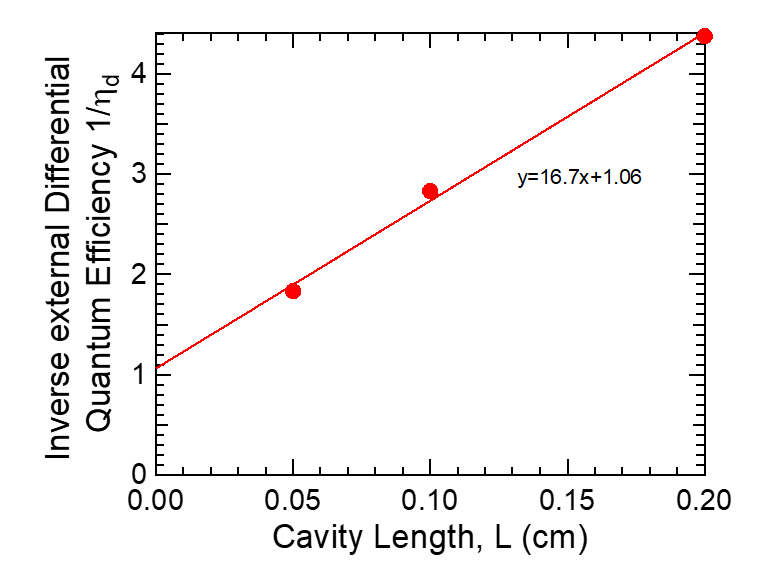
\includegraphics[width=10cm]{figure/fig_3_1_10QW_broadcontact_id_inverse.png}
	\caption{10QW外部量子効率の逆数}
	\label{fig:fig_3_1_10QW_broadcontact_id_inverse}
\end{figure}

\clearpage
\subsection{透明電流密度の見積もり}

次に透明電流密度$J_{0}$の見積もりを行った。共振器内の正味の利得$g_{\rm{net}}$は
\begin{eqnarray}
g_{\rm{net}}=\Gamma G-\alpha_{int}-\alpha_{m}
\label{eq:eta_j0}
\end{eqnarray}
と書ける。線形利得$G=g_{0}(J-J_{0})$を仮定すると閾値電流密度は
\begin{eqnarray}
J_{th}=J_{0}+\dfrac{\alpha_{int}}{\Gamma g_{0}}+\dfrac{1}{\Gamma g_{0}}\rm{ln}\left(\dfrac{1}{R}\right)\dfrac{1}{L}
\label{eq:j_th}
\end{eqnarray}
と書ける。この式にしたがうと$J_{\rm{th}}$は$1/L$に比例する。図\ref{fig:fig_3_1_3QW_broadcontact_j0}に$1/L$に対して$J_{\rm{th}}$をプロットした。色分けは共振器長を表す。
\begin{figure}[h]
	\centering
	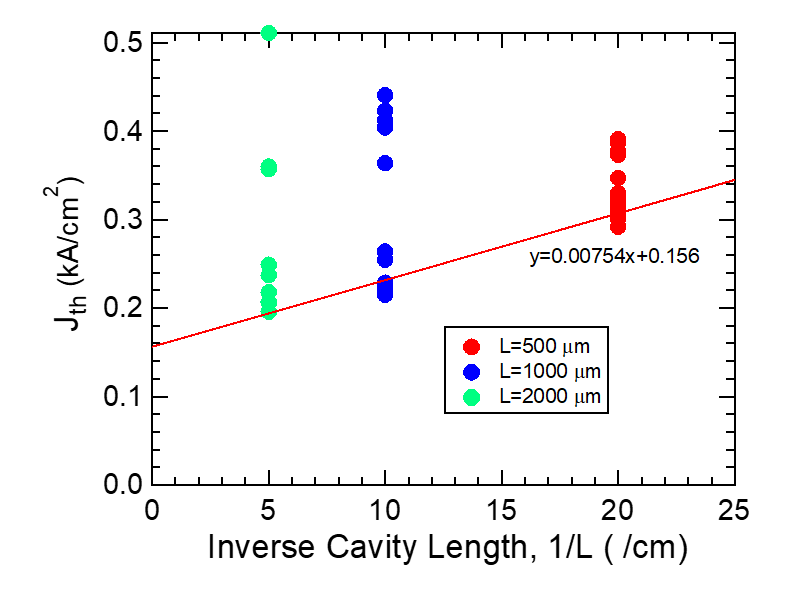
\includegraphics[width=10cm]{figure/fig_3_1_3QW_broadcontact_j0.png}
	\caption{3周期歪量子井戸ブロードコンタクトレーザーの透明電流密度の見積もり}
	\label{fig:fig_3_1_3QW_broadcontact_j0}
\end{figure}
図\ref{fig:fig_3_1_3QW_broadcontact_j0}のプロットのなかで、図\ref{fig:fig_3_1_3QW_broadcontact_Jth}において$J_{\rm{th}}$が一定となっているwが50以上のプロットに対して線形フィッティングを行った。赤い直線がフィッティング直線である。フィッティング結果から式(\ref{eq:j_th})の関係を用いて$\Gamma g_{0}$と$J_{0}$を見積もると$\Gamma g_{0}=151              \rm{ kA^{-1}}$、$J_{0}=0.0782 \rm{kA/cm^{2}}$を得た。


同様の解析を10周期歪補償量子井戸ブロードコンタクトレーザーについても行なった。図\ref{fig:fig_3_1_10QW_broadcontact_j0}に$J_{\rm{th}}$対$1/L$のプロットを示す。フィッティング結果から$\Gamma g_{0}$と$J_{0}$を見積もると$\Gamma g0=558   \rm{kA^{-1}}$、$J_{0}=0.357 \rm{kA/cm^{2}}$を得た。
\begin{figure}[t]
	\centering
	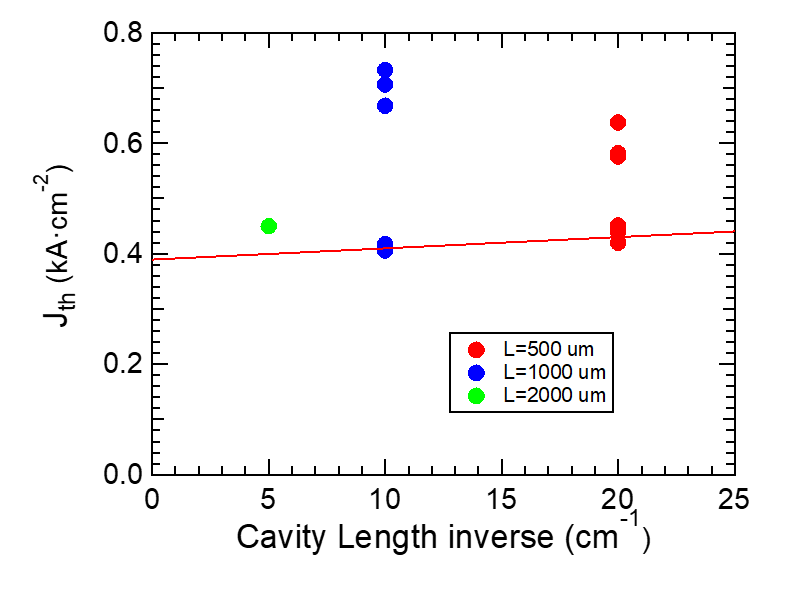
\includegraphics[width=10cm]{figure/fig_3_1_10QW_broadcontact_j0.png}
	\caption{10QWの透明電流密度の見積もり}
	\label{fig:fig_3_1_10QW_broadcontact_j0}
\end{figure}

\clearpage
\section{リッジ導波路型レーザーに関する実験結果}%===================
ブロードコンタクトレーザーを用い、半導体レーザーの基本的な特性を調べた。次に完成したデバイスとしてのリッジ導波路型レーザーに短パルス電流を印可し、利得スイッチング動作を行った。
\subsection{定常電流の結果}

利得スイッチング動作を行う前にまずは発振するか確かめること、および発振するならば閾値電流を見積もることを目的として定常電流による標準的なデバイス評価実験を行なった。方法はブロードコンタクトレーザーの評価測定と同じである。
\subsubsection{3周期歪量子井戸リッジ導波路型レーザーの結果}
まずは3周期歪量子井戸リッジ導波路型レーザーの結果を示す。2マイクロ秒パルスを2ミリ秒周期で印可した。デューティー比は1:1000である。
まずは3周期歪量子井戸リッジ導波路型レーザーの結果を図\ref{fig:fig_3_2_3QW_ridge_IL}に示す。図\ref{fig:fig_3_2_3QW_ridge_IL}(a)はILカーブ、(b)はIVカーブである。色分けは共振器長Lの違いを表す。

\begin{figure}[h]
	\centering
	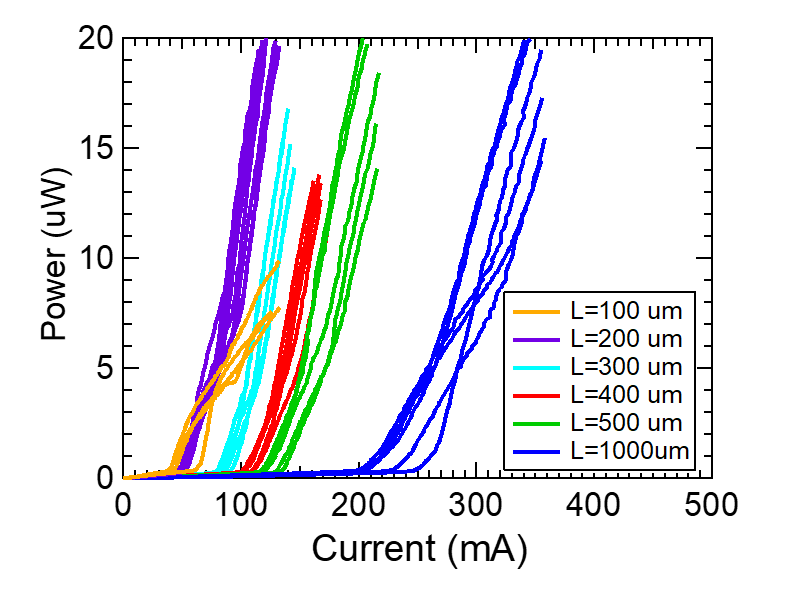
\includegraphics[width=15cm]{figure/fig_3_2_3QW_ridge_IL.png}
		\caption{3周期歪量子井戸リッジ導波路型レーザーのILカーブおよびIVカーブ}
		\label{fig:fig_3_2_3QW_ridge_IL}
\end{figure}


次にILカーブから見積もった閾値電流$I_{\rm{th}}$、$J_{\rm{th}}$と閾値電流密度を図\ref{fig:fig_3_2_3QW_ridge_Ith}に示す。図中の丸プロットが閾値電流$I_{\rm{th}}$であり左の軸に対してのプロットした。十字プロットは閾値電流を共振器長とリッジ幅の積で割った値の閾値電流密度$J_{\rm{th}}$であり右の軸に対してのプロットである。横軸は共振器長である。色分けはリッジ幅の違いを表している。紫がリッジ幅1.5 um、黄色が2.5 umである。

これを見ると閾値電流は共振器長に対して概ね線形に増加しており最短では50mA程度となっている。またリッジ幅の差異に対する差異が見られていない。これは電流が広がってしまっているためだと考えられる。

閾値電流密度はLが300より大きい共振器長において概ね横ばいとなっており10から20 $\rm{kA/cm^2}$の値を持っている。


\begin{figure}[h]
	\centering
	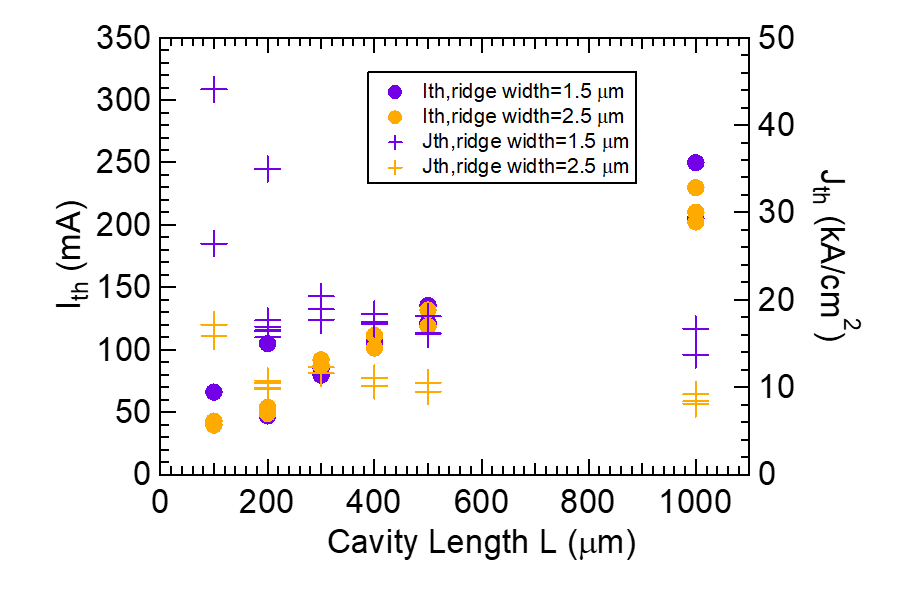
\includegraphics[width=10cm]{figure/fig_3_2_3QW_ridge_Ith.png}
		\caption{3周期歪量子井戸リッジ導波路型レーザーの$I_{\rm{th}}$、$J_{\rm{th}}$}
		\label{fig:fig_3_2_3QW_ridge_Ith}
\end{figure}
次にILカーブの発振領域の発光効率$2 \Delta P/\Delta I$および外部量子効率$\eta_{\rm{d}}$を共振器長に対してプロットした結果を図\ref{fig:fig_3_2_3QW_ridge_slope}に示す。
\begin{figure}[h]
	\centering
	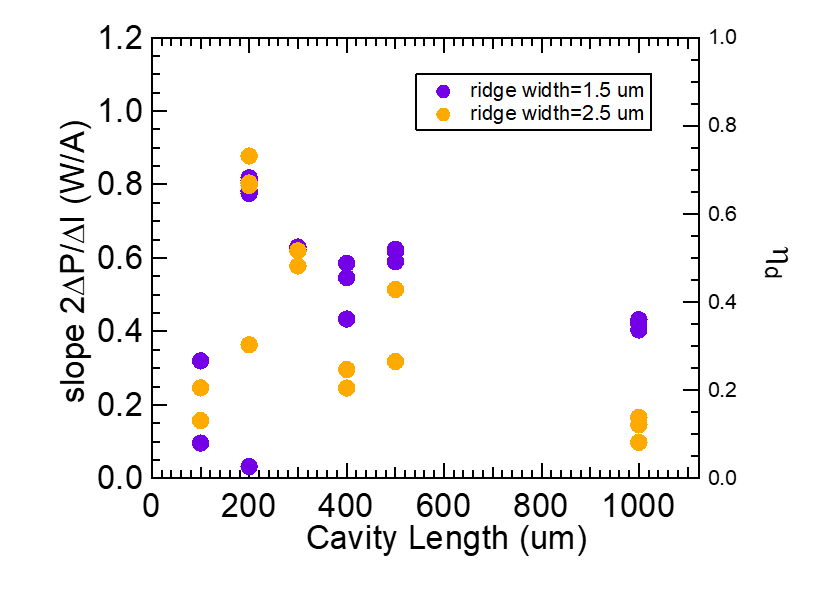
\includegraphics[width=10cm]{figure/fig_3_2_3QW_ridge_slope.png}
		\caption{3周期歪量子井戸リッジ導波路型レーザーのスロープおよび微分外部量子効率}
		\label{fig:fig_3_2_3QW_ridge_slope}
\end{figure}

\clearpage
\subsubsection{10周期歪補償量子井戸リッジ導波路レーザー}
次に10周期歪補償量子井戸リッジ導波路レーザーの結果を示す。図\ref{fig:fig_3_2_10QW_ridge_IL}(a)にILカーブ、(b)にIVカーブを示す。

\ref{fig:fig_3_2_10QW_ridge_IL}(a)を見るとそれぞれの共振器長において発振したことがわかる。L=400umの赤い線を見るとI=200mA付近からどの試料においても発光量が下がってきている。
\begin{figure}[h]
	\centering
	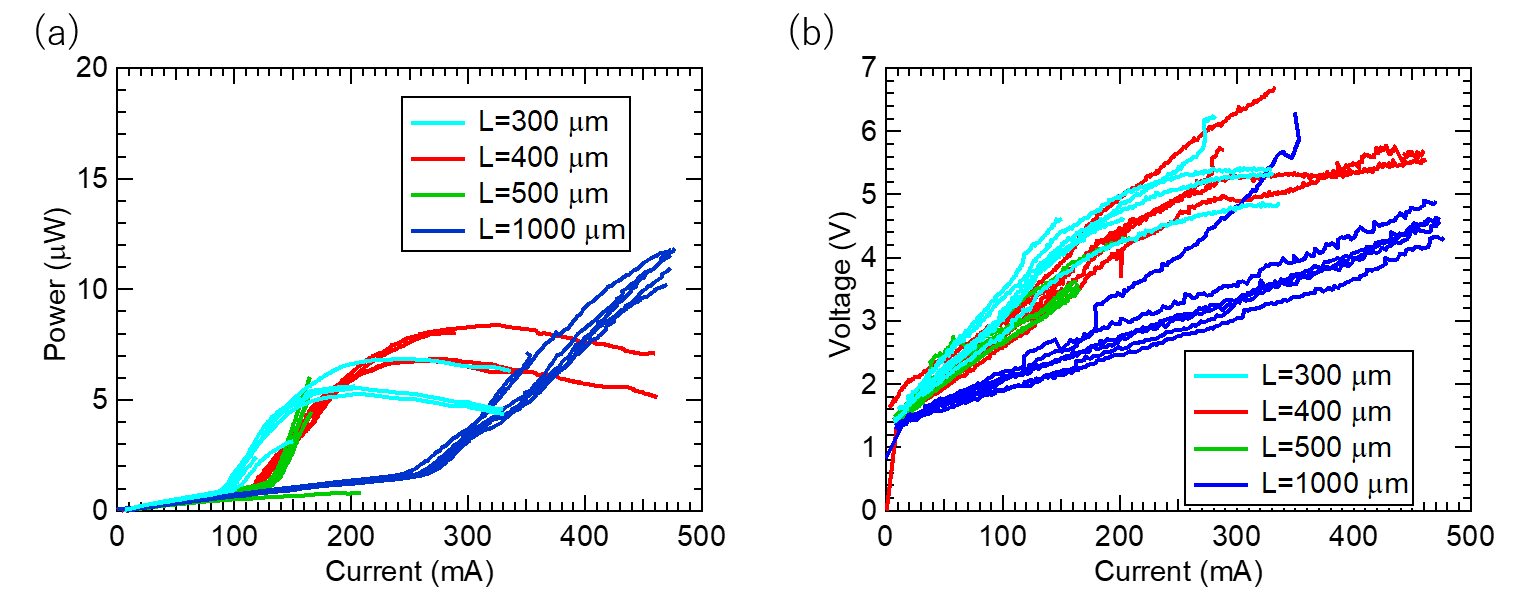
\includegraphics[width=15cm]{figure/fig_3_2_10QW_ridge_IL.png}
		\caption{10周期 リッジ導波路型レーザーのILカーブおよびIVカーブ}
		\label{fig:fig_3_2_10QW_ridge_IL}
\end{figure}
次にILカーブから閾値電流$I_{\rm{th}}$と閾値電流密度$J_{\rm{th}}$を出した。その結果を図\ref{fig:fig_3_2_10QW_ridge_Ith}に示す。閾値電流は共振器長に対して線形に増加しており最小で90mA程度となった。色分けはリッジ幅の違いを表すが、閾値電流においてリッジ幅の際は見られない。閾値電流密度は10から20$\rm{kA/cm^{2}}$程度となった。
\begin{figure}[h]
	\centering
	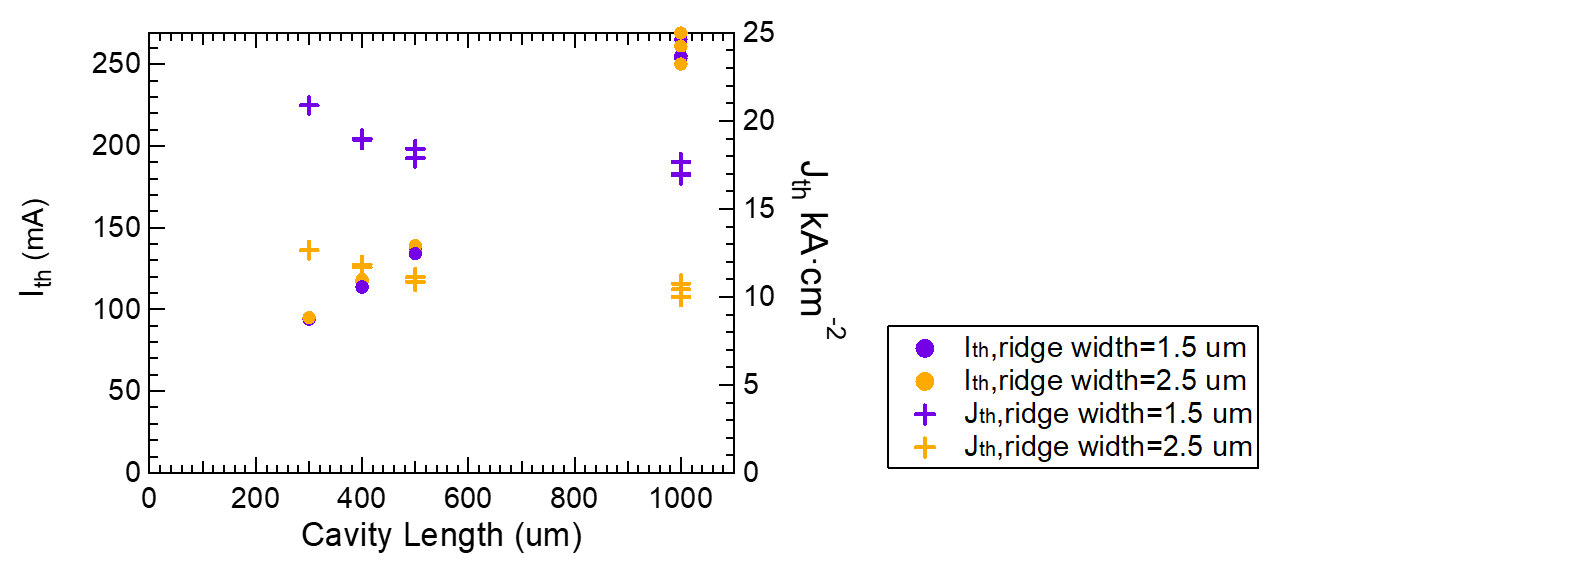
\includegraphics[width=10cm]{figure/fig_3_2_10QW_ridge_Ith.png}
		\caption{10周期歪補償量子井戸リッジ導波路型レーザーの閾値電流と閾値電流密度}
		\label{fig:fig_3_2_10QW_ridge_Ith}
\end{figure}
ILカーブの発振時の傾きから見積もったスロープ効率$2\Delta P/\Delta I$および外部微分量子効率$\eta_{\rm{d}}$を図\ref{fig:fig_3_2_10QW_ridge_slope}に示す。
\begin{figure}[h]
	\centering
	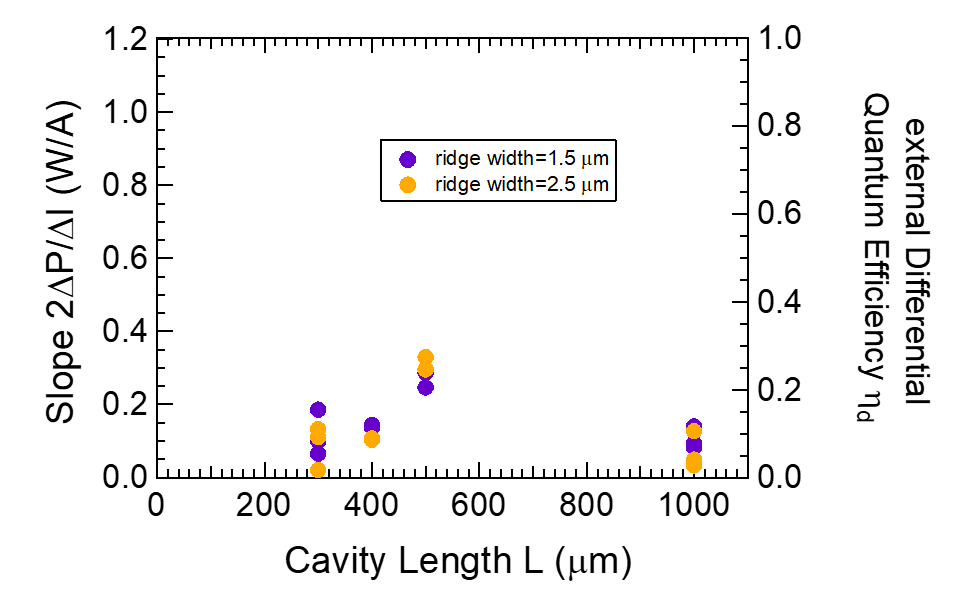
\includegraphics[width=10cm]{figure/fig_3_2_10QW_ridge_slope.png}
		\caption{10周期歪補償量子井戸リッジ導波路型レーザーのスロープおよび外部微分量子効率}
		\label{fig:fig_3_2_10QW_ridge_slope}
\end{figure}
\clearpage
\subsection{短パルス電流注入の結果}
リッジ導波路型レーザーに関して電流注入利得スイッチング実験を行った。そのILと時間波形を示す。
\subsection{IL}
10周期と3周期一個づつ
\begin{figure}[h]
	\centering
	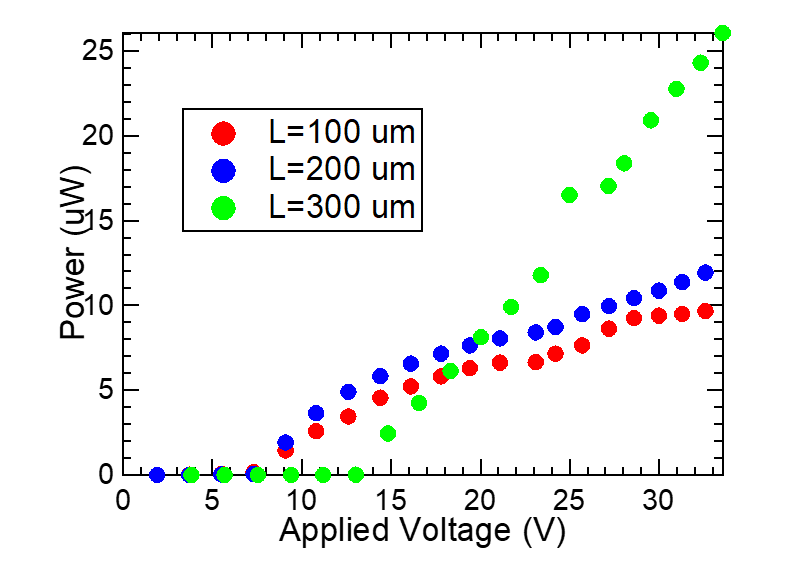
\includegraphics[width=15cm]{figure/fig_3_2_3QW_ridge_GS_power.png}
		\caption{3MQW 短パルス駆動時のILカーブ}
		\label{fig:fig_3_2_3QW_ridge_GS_power}
\end{figure}

\begin{figure}[h]
	\centering
	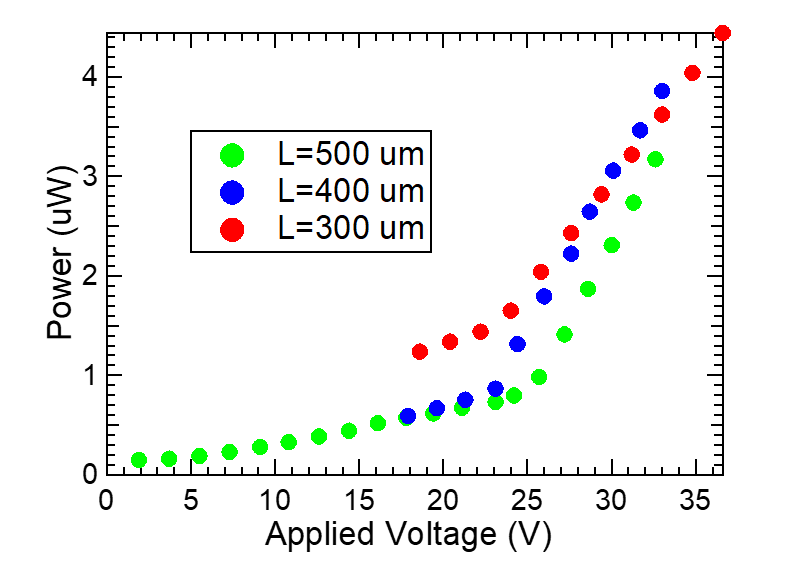
\includegraphics[width=15cm]{figure/fig_3_2_10QW_ridge_GS_power.png}
		\caption{10MQW 短パルス駆動時のILカーブ}
		\label{fig:fig_3_2_10QW_ridge_GS_power}
\end{figure}
\clearpage
\subsection{3QW試料の利得スイッチング動作}%===============================
時間波形を示す。図\ref{fig:fig_3_2_3QW_ridge_L100_GS}(a)に3周期量子井戸レーザーの励起強度を変えたときの時間波形を示す。図\ref{fig:fig_3_2_3QW_ridge_L100_GS}(b)には強度を規格化したプロットをしめす。これらを見ると励起強度を大きくするに従ってピーク強度が高くなっていき、また立ち上がりが早くなっていることがわかる。
\begin{figure}[h]
	\centering
	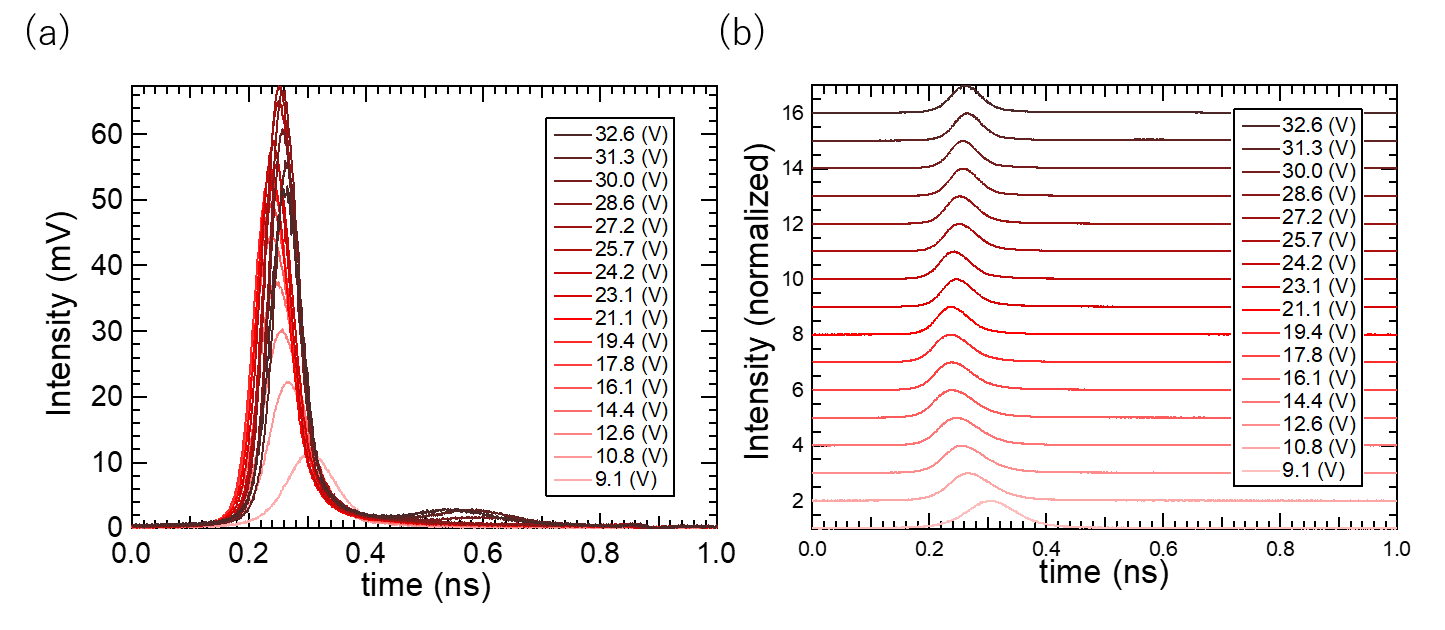
\includegraphics[width=15cm]{figure/fig_3_2_3QW_ridge_L100_GS.png}
		\caption{3MQW L=100um の利得スイッチング光パルスの時間波形}
		\label{fig:fig_3_2_3QW_ridge_L100_GS}
\end{figure}

\begin{figure}[h]
	\centering
	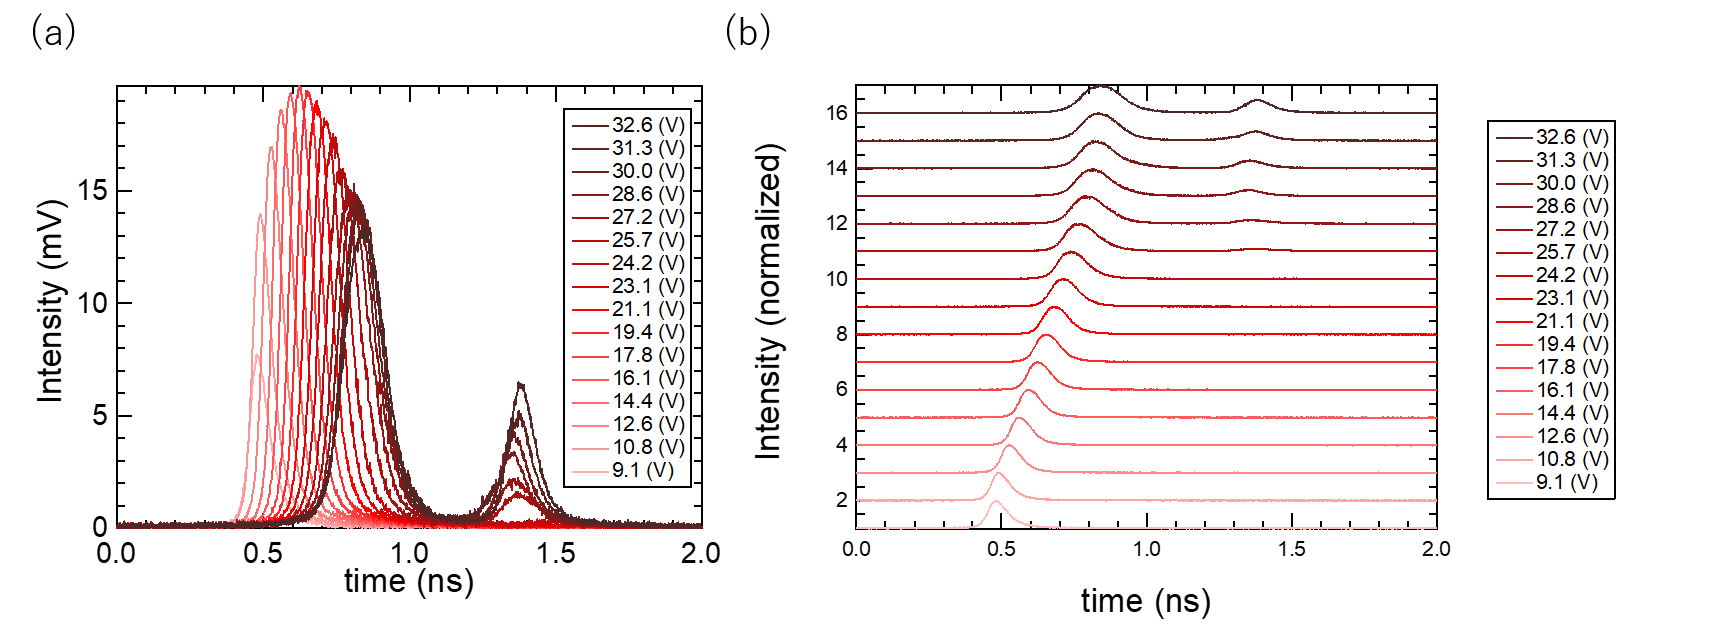
\includegraphics[width=15cm]{figure/fig_3_2_3QW_ridge_L200_GS.png}
		\caption{3MQW L=200um の利得スイッチング光パルスの時間波形}
		\label{fig:fig_3_2_3QW_ridge_L200_GS}
\end{figure}
\begin{figure}[h]
	\centering
	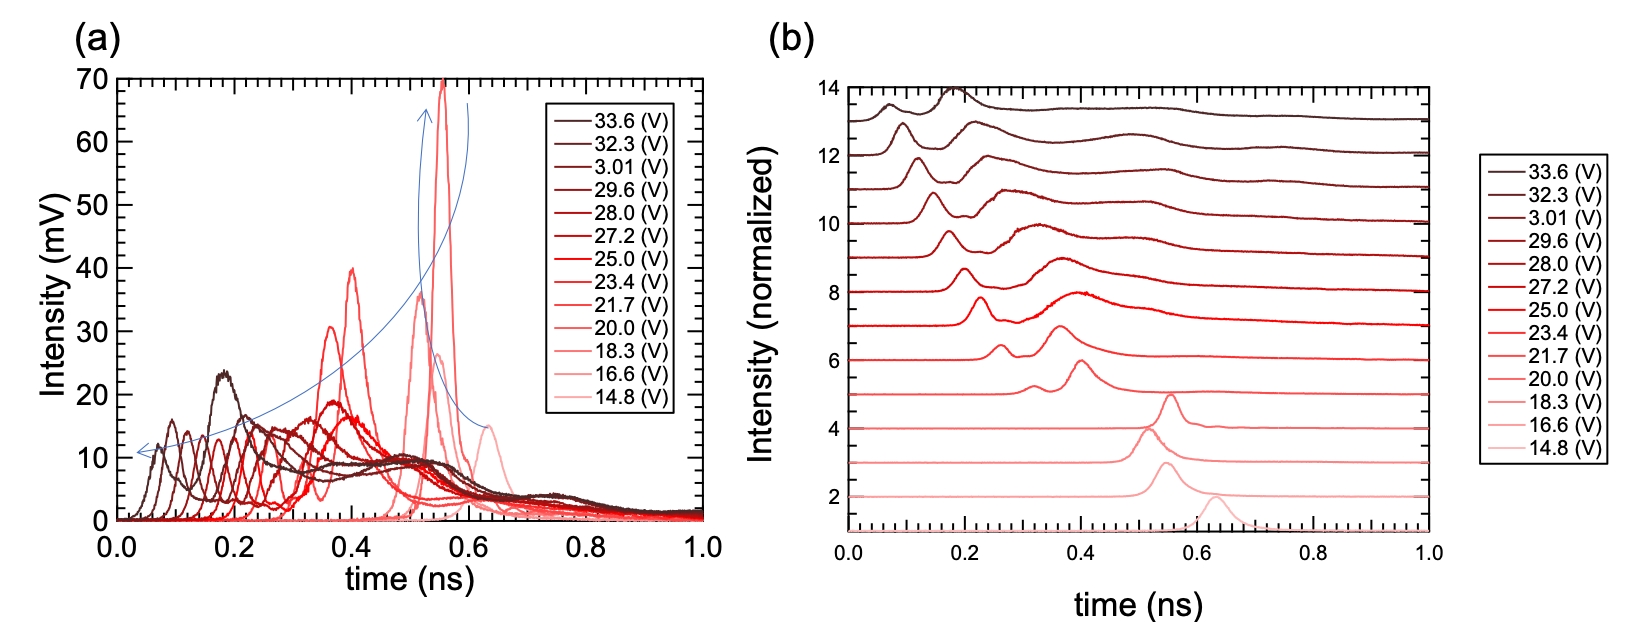
\includegraphics[width=15cm]{figure/fig_3_2_3QW_ridge_L300_GS.png}
		\caption{3MQW L=300um の利得スイッチング光パルスの時間波形}
		\label{fig:fig_3_2_3QW_ridge_L300_GS}
\end{figure}
\newpage
\clearpage
\subsection{10QW試料の利得スイッチング動作}%==============================
L=300,400,500
\begin{figure}[h]
	\centering
	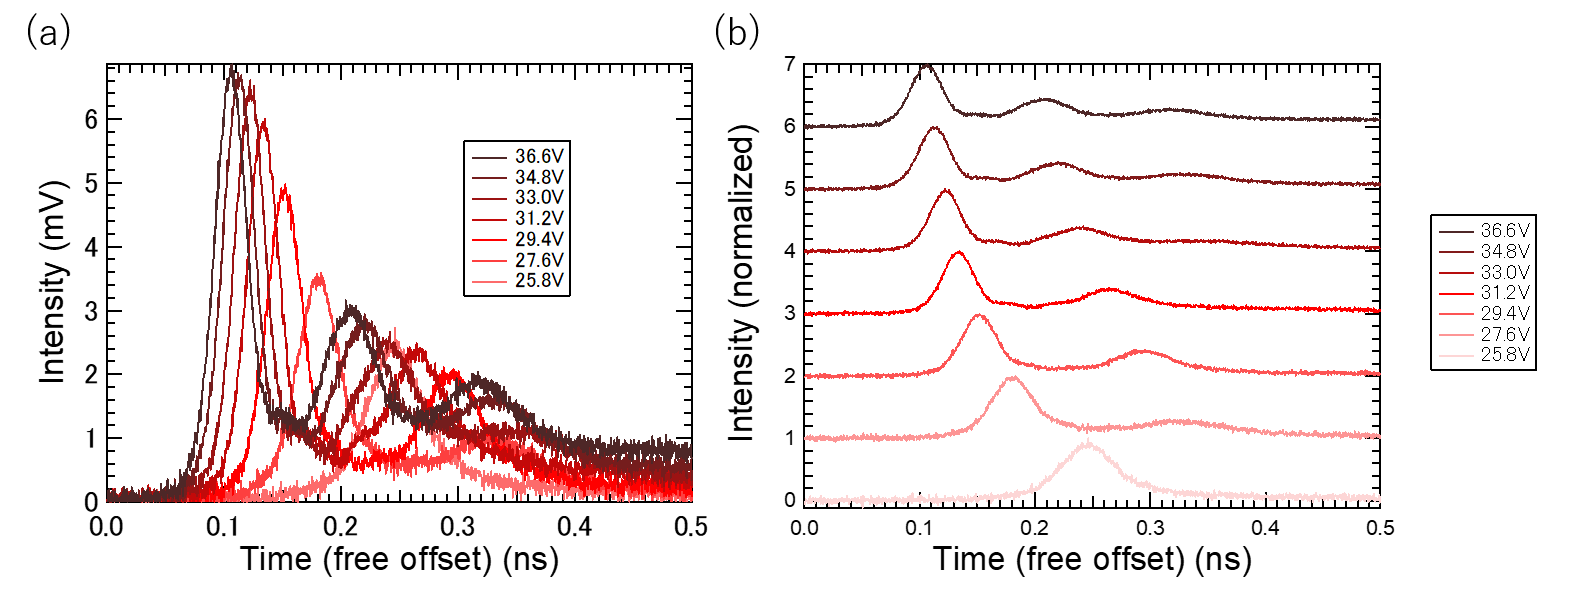
\includegraphics[width=15cm]{figure/fig_3_2_10QW_ridge_L300_GS.png}
		\caption{10MQW L=300um の利得スイッチング光パルスの時間波形}
		\label{fig:fig_3_2_10QW_ridge_L300_GS}
\end{figure}

\begin{figure}[h]
	\centering
	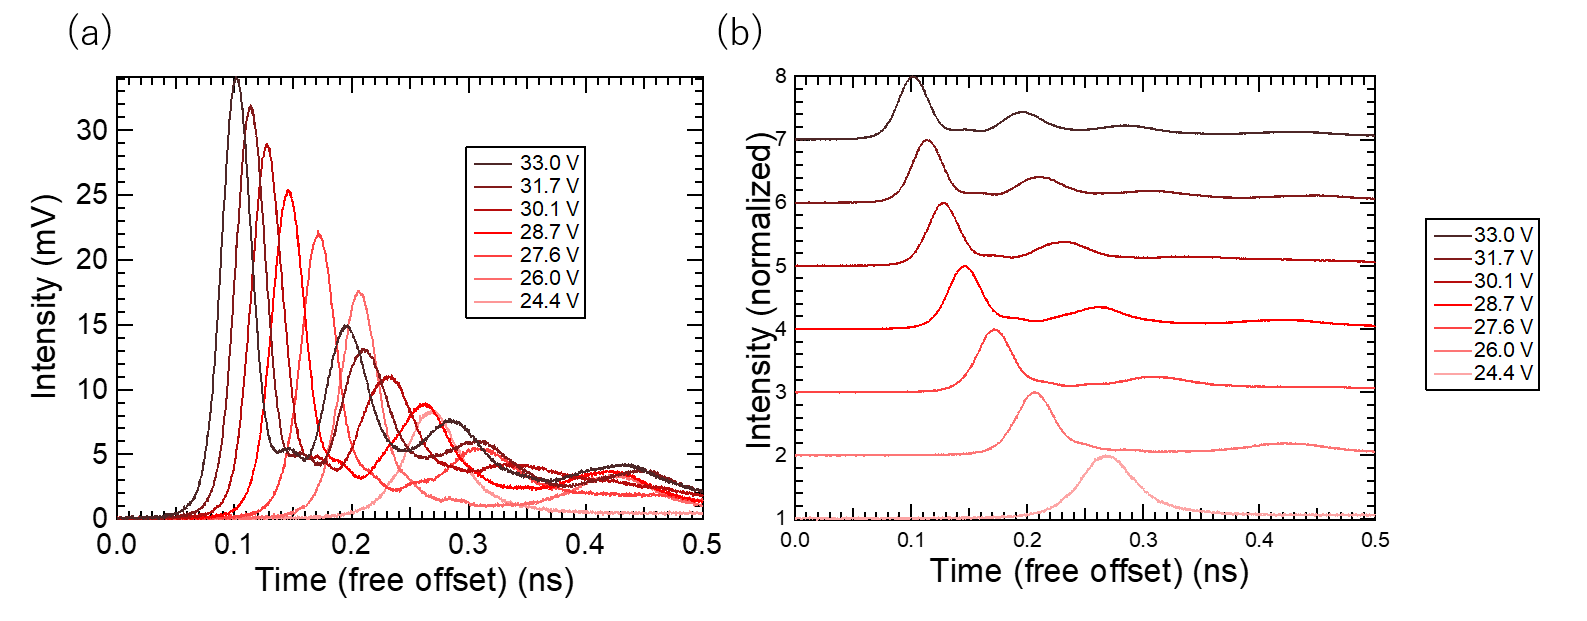
\includegraphics[width=15cm]{figure/fig_3_2_10QW_ridge_L400_GS.png}
		\caption{10MQW L=400um の利得スイッチング光パルスの時間波形}
		\label{fig:fig_3_2_10QW_ridge_L400_GS}
\end{figure}
\begin{figure}[h]
	\centering
	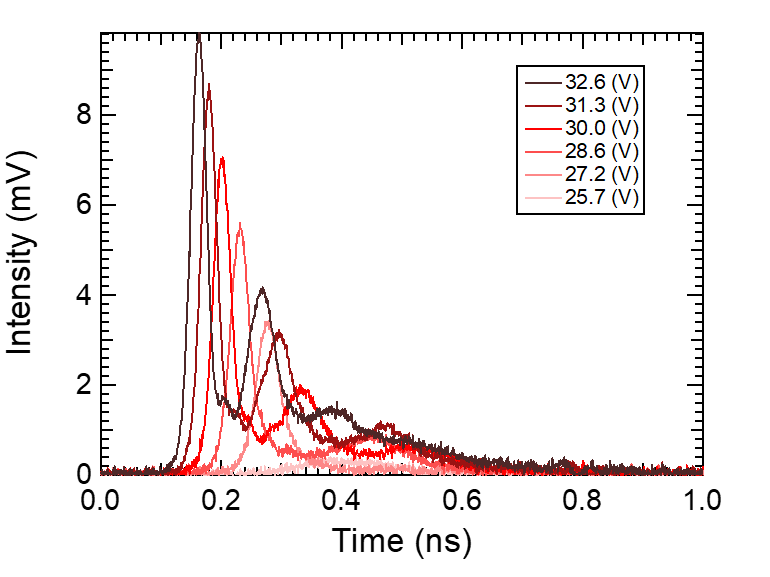
\includegraphics[width=15cm]{figure/fig_3_2_10QW_ridge_L500_GS.png}
		\caption{10MQW L=500um の利得スイッチング光パルスの時間波形}
		\label{fig:fig_3_2_10QW_ridge_L500_GS}
\end{figure}
\clearpage
\subsection{結果の比較}%===========================
FWHM をまとめた。でコンボリューション後の値を示した。
\begin{figure}[h]
	\centering
	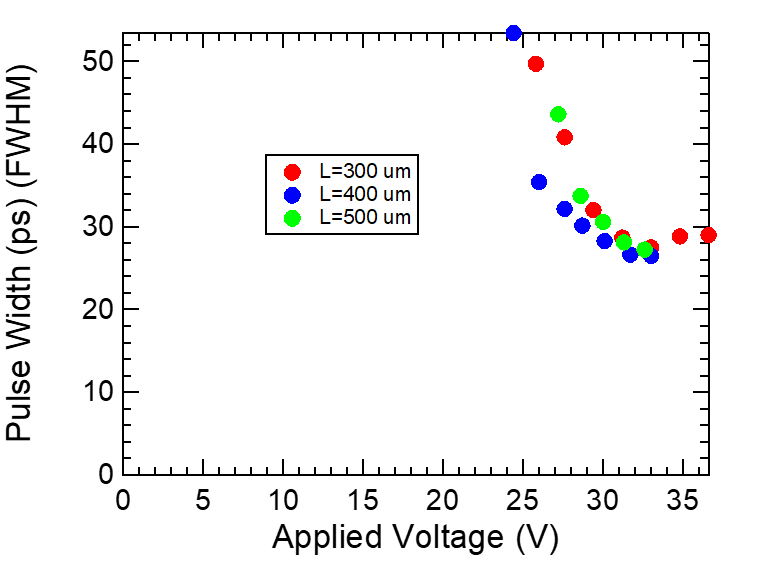
\includegraphics[width=10cm]{figure/fig_3_2_10QW_ridge_GS_FWHM.png}
		\caption{10MQW 利得スイッチングパルスのパルス幅}
		\label{fig:fig_3_2_10QW_ridge_GS_FWHM}
\end{figure}

\begin{figure}[h]
	\centering
	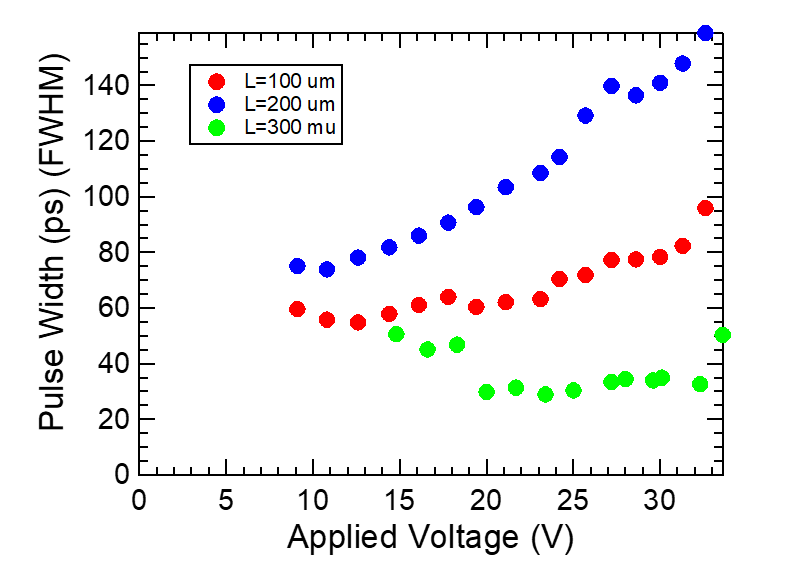
\includegraphics[width=10cm]{figure/fig_3_2_3QW_ridge_GS_FWHM.png}
		\caption{3MQW 利得スイッチングパルスのパルス幅}
		\label{fig:fig_3_2_3QW_ridge_GS_FWHM}
\end{figure}
\clearpage 
%\subsection{付録かな??コンボリュージョンの説明,電気パルスの確認}%==============
\begin{comment}
\begin{figure}[h]
	\centering
	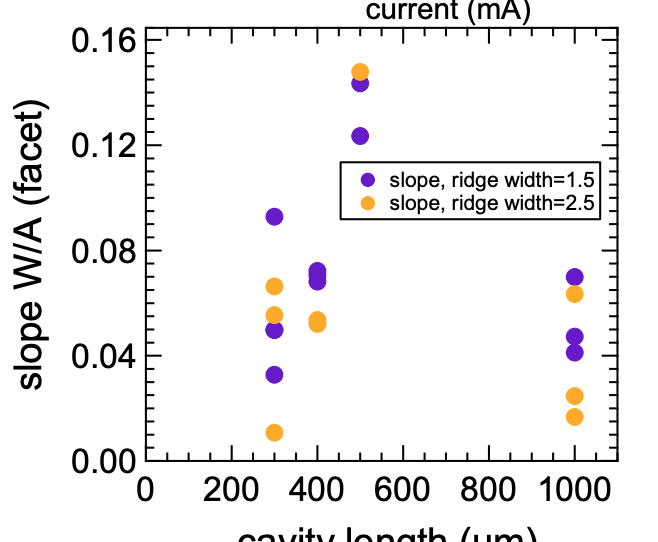
\includegraphics[width=10cm]{figure/fig_3_1_broad_slope_10QW.png}
		\caption{10MQWのスロープ}
		\label{fig_3_1_IL_broad_slope}
\end{figure}

\begin{figure}[h]
	\centering
	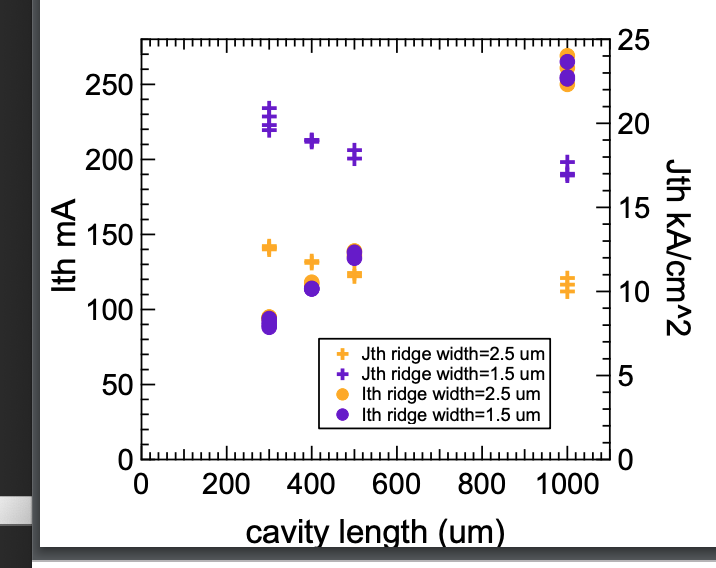
\includegraphics[width=10cm]{figure/fig_3_1_broad_i_th_10QW.png}
		\caption{10MQWの閾値電流}
		\label{fig_3_1_broad_i_th_3QW}
\end{figure}


\begin{figure}[h]
	\centering
	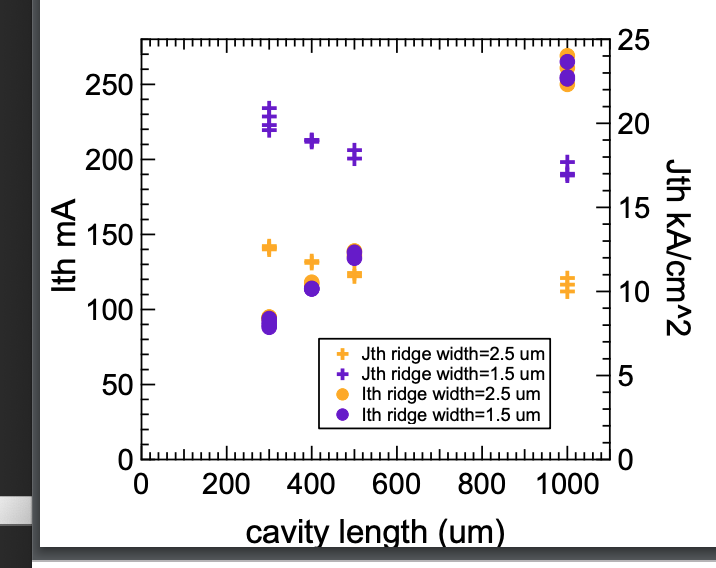
\includegraphics[width=10cm]{figure/fig_3_1_broad_i_th_10QW.png}
		\caption{10MQWの閾値電流密度のパッド幅依存性}
		\label{fig_3_1_broad_j_th_10QW}
\end{figure}
\end{comment}
\section{考察}%========================================

\subsection{自然放出光?}
\subsection{閾値電流}
\subsection{利得スイッチングパルスのパルス幅の比較}
